\documentclass[a4paper,12pt]{article}
%%%%%%%%%%%%%%%%%%%%%%%%%%%%%%%%%%%%%%%%%%%%%%%%%%%%%%%%%%%%%%%%%%%%%%%%%%%%%%%%%%%%%%%%%%%%%%%%%%%%%%%%%%%%%%%%%%%%%%%%%%%%%%%%%%%%%%%%%%%%%%%%%%%%%%%%%%%%%%%%%%%%%%%%%%%%%%%%%%%%%%%%%%%%%%%%%%%%%%%%%%%%%%%%%%%%%%%%%%%%%%%%%%%%%%%%%%%%%%%%%%%%%%%%%%%%
\usepackage{eurosym}
\usepackage{vmargin}
\usepackage{amsmath}
\usepackage{graphics}
\usepackage{epsfig}
\usepackage{framed}
\usepackage{subfigure}
\usepackage{fancyhdr}

\setcounter{MaxMatrixCols}{10}
%TCIDATA{OutputFilter=LATEX.DLL}
%TCIDATA{Version=5.00.0.2570}
%TCIDATA{<META NAME="SaveForMode"CONTENT="1">}
%TCIDATA{LastRevised=Wednesday, February 23, 201113:24:34}
%TCIDATA{<META NAME="GraphicsSave" CONTENT="32">}
%TCIDATA{Language=American English}

\pagestyle{fancy}
\setmarginsrb{20mm}{0mm}{20mm}{25mm}{12mm}{11mm}{0mm}{11mm}
\lhead{MA4128} \rhead{Kevin O'Brien} \chead{Week 8 Part B} %\input{tcilatex}

%http://www.electronics.dit.ie/staff/ysemenova/Opto2/CO_IntroLab.pdf
\begin{document}
	
	\tableofcontents
	\newpage
	

%-------------------------------------------------------------- %
	\section{Residual}
	
	A residual (or fitting error), on the other hand, is an observable estimate of the unobservable statistical error.
	Residual (or error) represents unexplained (or residual) variation after fitting a regression model. It is the difference (or left over) between the observed value of the variable and the value suggested by the regression model.
	Consider the previous example with men's heights and suppose we have a random sample of n people. The sample mean could serve as a good estimator of the population mean. Then we have:
	
	
	The difference between the observed value of the dependent variable (y) and the predicted value (ŷ) is called the residual (e). Each data point has one residual.
	
	\[ \mbox{Residual} = \mbox{Observed value} - \mbox{Predicted value}\]
	\[e = y - \hat{y} \]
	
	Both the sum and the mean of the residuals are equal to zero. .
	
	%--------------------------------- %
	
	
	The difference between the height of each man in the sample and the unobservable population mean is a statistical error, whereas
	The difference between the height of each man in the sample and the observable sample mean is a residual.
	Note that the sum of the residuals within a random sample is necessarily zero, and thus the residuals are necessarily not independent. The statistical errors on the other hand are independent, and their sum within the random sample is almost surely not zero.
	
	%------------------------------- %
	
\subsection{Other uses of the word "error" in statistics}
	
	The use of the term "error" as discussed in the sections above is in the sense of a deviation of a value from a hypothetical unobserved value. At least two other uses also occur in statistics, both referring to observable prediction errors:
	
	\begin{itemize}
		\item Mean square error or mean squared error (abbreviated MSE) and root mean square error (RMSE) refer to the amount by which the values predicted by an estimator differ from the quantities being estimated (typically outside the sample from which the model was estimated).
		
		\item 
		Sum of squared errors, typically abbreviated SSE or SSe, refers to the residual sum of squares (the sum of squared residuals) of a regression; this is the sum of the squares of the deviations of the actual values from the predicted values, within the sample used for estimation. Likewise, the sum of absolute errors (SAE) refers to the sum of the absolute values of the residuals, which is minimized in the least absolute deviations approach to regression.
		
	\end{itemize}
	
	%=================================================== %
	% http://www.ime.usp.br/~jmsinger/MAE0610/Mixedmodelresiduals.pdf
	\subsection{Residual Plots}
	A residual plot is a graph that shows the residuals on the vertical axis and the independent variable on the horizontal axis. If the points in a residual plot are randomly dispersed around the horizontal axis, a linear regression model is appropriate for the data; otherwise, a non-linear model is more appropriate.
	
	Below the table on the left shows inputs and outputs from a simple linear regression analysis, and the chart on the right displays the residual (e) and independent variable (X) as a residual plot.
	
	%x	60	70	80	85	95
	%y	70	65	70	95	85
	%ŷ	65.411	71.849	78.288	81.507	87.945
	%e	4.589	-6.849	-8.288	13.493	-2.945
	% Image of residual plot
	
	The residual plot shows a fairly random pattern - the first residual is positive, the next two are negative, the fourth is positive, and the last residual is negative. This random pattern indicates that a linear model provides a decent fit to the data.
	
	Below, the residual plots show three typical patterns. The first plot shows a random pattern, indicating a good fit for a linear model. The other plot patterns are non-random (U-shaped and inverted U), suggesting a better fit for a non-linear model.
	
	
	%Random pattern	Non-random: U-shaped	Non-random: Inverted U
	In the next lesson, we will work on a problem, where the residual plot shows a non-random pattern. And we will show how to "transform" the data to use a linear model with nonlinear data.
	\section{Studentization}
	In statistics, a studentized residual is the quotient resulting from the division of a residual by an estimate of its standard deviation. Typically the standard deviations of residuals in a sample vary greatly from one data point to another even when the errors all have the same standard deviation, particularly in regression analysis; thus it does not make sense to compare residuals at different data points without first studentizing. It is a form of a Student's t-statistic, with the estimate of error varying between points.
	
	This is an important technique in the detection of outliers. It is named in honor of William Sealey Gosset, who wrote under the pseudonym Student, and dividing by an estimate of scale is called studentizing, in analogy with standardizing and normalizing: see Studentization.
	
	\section{Residual Analysis for LME Models}
	
	In classical linear models model diagnostics have been become a required part of any statistical analysis, and the methods are commonly available in statistical packages and standard textbooks on applied regression. However it has been noted by several papers that model diagnostics do not often accompany LME model analyses.
	
	\textbf{Cite:Zewotir} lists several established methods of analyzing influence in LME models. These methods include \begin{itemize}
		\item Cook's distance for LME models,
		\item \index{likelihood distance} likelihood distance,
		\item the variance (information) ration,
		\item the \index{Cook-Weisberg statistic} Cook-Weisberg statistic,
		\item the \index{Andrews-Prebigon statistic} Andrews-Prebigon statistic.
	\end{itemize}
	
	
	
	
	%--------------------------------------------------------------%
	\subsection{LME REsiduals}	
	Cox and Snell (1968, JRSS-B): general definition of residuals for
	models with single source of variability
	Hilden-Minton (1995, PhD thesis UCLA), Verbeke and Lesaffre
	(1997, CSDA) or Pinheiro and Bates (2000, Springer): extension to
	define three types of residuals that accommodate the extra source of
	variability present in linear mixed models, namely:
	
	i) Marginal residuals, 
	%bξ = y − X\hat{\beta} = \hat{M}^{-1}\hat{Q}y ,
	
	predictors of marginal errors, 
	
	%ξ = y − E[y] = y − X\beta = Zb + e
	
	ii) Conditional residuals, 
	\[be = y − X\hat{\beta} − Zbb = \hat{\sigma}Q\hat{y}\] , predictors of
	conditional errors 
	\[e = y − E[y|b] = y − X\beta − Zb\]
	
	iii) BLUP, Zbb, predictors of random effects,
	\[ Zb = E[y|b] − E[y]\]
	

	%----------------------------- %
	\section{Residual Diagnostics}
	
	Consider a residual vector of the form $\hat{e} = \boldsymbol{PY} $, where $\boldsymbol{P}$ is a projection matrix, possibly an oblique projector.
	External studentization uses an estimate of $Var$ that does not involve the $i$th observation.
	
	Externally studentized residuals are often preferred over studentized residuals because they have well known distributional
	properties in the standard linear models for independent data.
	
	Residuals that are scaled by the estimated variances of the responses are referred to as Pearson-type residuals.
	
	Standardization: \[ \frac{\hat{e}_i}{\sqrt{v_i}}\]
	Studentization \[ \frac{\hat{e}_i}{\sqrt{\hat{v}_i}}\]
	


	
	

	\section{residuals.lme {nlme}- Extract lme Residuals}
	
	The residuals at level $i$ are obtained by subtracting the fitted levels at that level from the response vector (and dividing by the estimated within-group standard error, if \texttt{type="pearson"}). 
	
	The fitted values at level i are obtained by adding together the population fitted values (based only on the fixed effects estimates) and the estimated contributions of the random effects to the fitted values at grouping levels less or equal to i.
	
	%------------------------------------------------------------------------%
	
	\begin{framed}
		\begin{verbatim}
		
		fm1 <- lme(distance ~ age + Sex, 
		data = Orthodont, random = ~ 1)
		head(residuals(fm1, level = 0:1))
		summary(residuals(fm1) /
		residuals(fm1, type = "p")) 
		
		# constant scaling factor 1.432
		
		\end{verbatim}
	\end{framed}
	
	%-------------------------------------------------------------------------------------------------------------------------------------%
\section{Diagnostic Plots for Linear Models with \texttt{R}}
Plot Diagnostics for an \texttt{lm} Object

%% \subsection{Description}

Six plots (selectable by \texttt{which}) are currently available: 
\begin{enumerate}
	\item a plot of residuals against fitted values, 
	\item a Scale-Location plot of \textit{sqrt(| residuals |}) against fitted values, 
	\item a Normal Q-Q plot, 
	\item a plot of Cook's distances versus row labels, 
	\item a plot of residuals against leverages, 
	\item a plot of Cook's distances against leverage/(1-leverage).
\end{enumerate} By default, the first three and 5 are provided.
	%====================================================================%
	\subsubsection{Residuals plots}
	
	lme allows to plot the residuals in the following ways:
	
	\begin{framed}
		\begin{verbatim}
		res_lme=residuals(model_lme)
		plot(res_lme)
		qqnorm(res_lme)
		qqline(res_lme)
		plot(model_lme)
		\end{verbatim}
	\end{framed}
	
	When the \texttt{plot} function calls the model object, the residual plot is produced.
	
	
	%====================================================================%
	
	
	\begin{framed}
		\begin{verbatim}
		plot(JS.roy1, which=c(1) )
		\end{verbatim}
	\end{framed}
	
	LME models assume that the residuals of the model are normally distributed. A Normal probability plot can be constructed to check this assumption. Commonly used \texttt{R} commands can be used to construct the plot.
	
	
	\begin{framed}
		\begin{verbatim}
		qqnorm(resid(JS.roy1),pch="*",col="red")
		qqline(resid(JS.roy1),col="blue")
		\end{verbatim}
	\end{framed}
	
	\begin{framed}
		\begin{verbatim}
		table(dat$method[1:255])
		## 
		##   J   S 
		## 255   0
		table(dat$method[256:510])
		## 
		##   J   S 
		##   0 255
		\end{verbatim}	
	\end{framed}
	\begin{framed}
		\begin{verbatim}
		library(predictMeans)
		CookD(model, group=method, plot=TRUE, idn=5, newwd=FALSE)
		\end{verbatim}
	\end{framed}
	
	
	
	
	
	
	\begin{framed}
		\begin{verbatim}
		> shapiro.test(resid(JS.roy1)[256:510])
		
		Shapiro-Wilk normality test
		
		data:  resid(JS.roy1)[256:510]
		W = 0.9395, p-value = 9.503e-09
		\end{verbatim}
	\end{framed}
	%	\begin{figure}[h!]
	%		\centering
	%		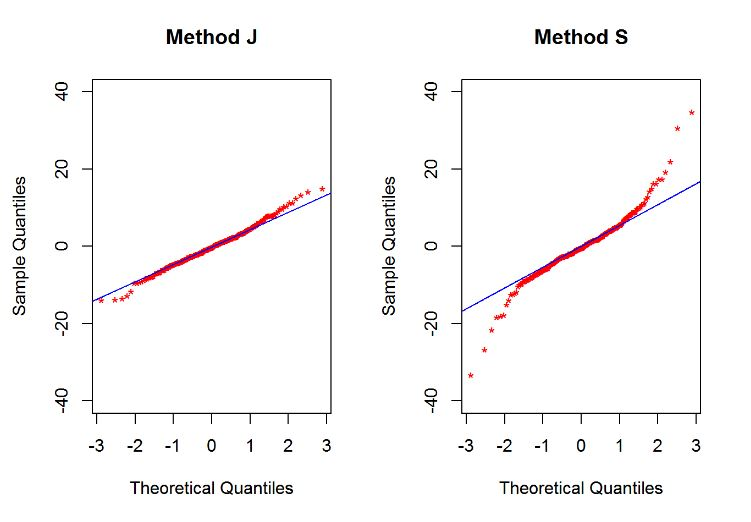
\includegraphics[width=0.9\linewidth]{images/Resid-newplot2}
	%		
	%	\end{figure}
	
	\begin{framed}
		\begin{verbatim}
		plot(roy.NLME, resid(., type = "p") ~ fitted(.) | method, 
		abline = 0, id=.05)
		\end{verbatim}
	\end{framed}
	%	\begin{figure}
	%		\centering
	%		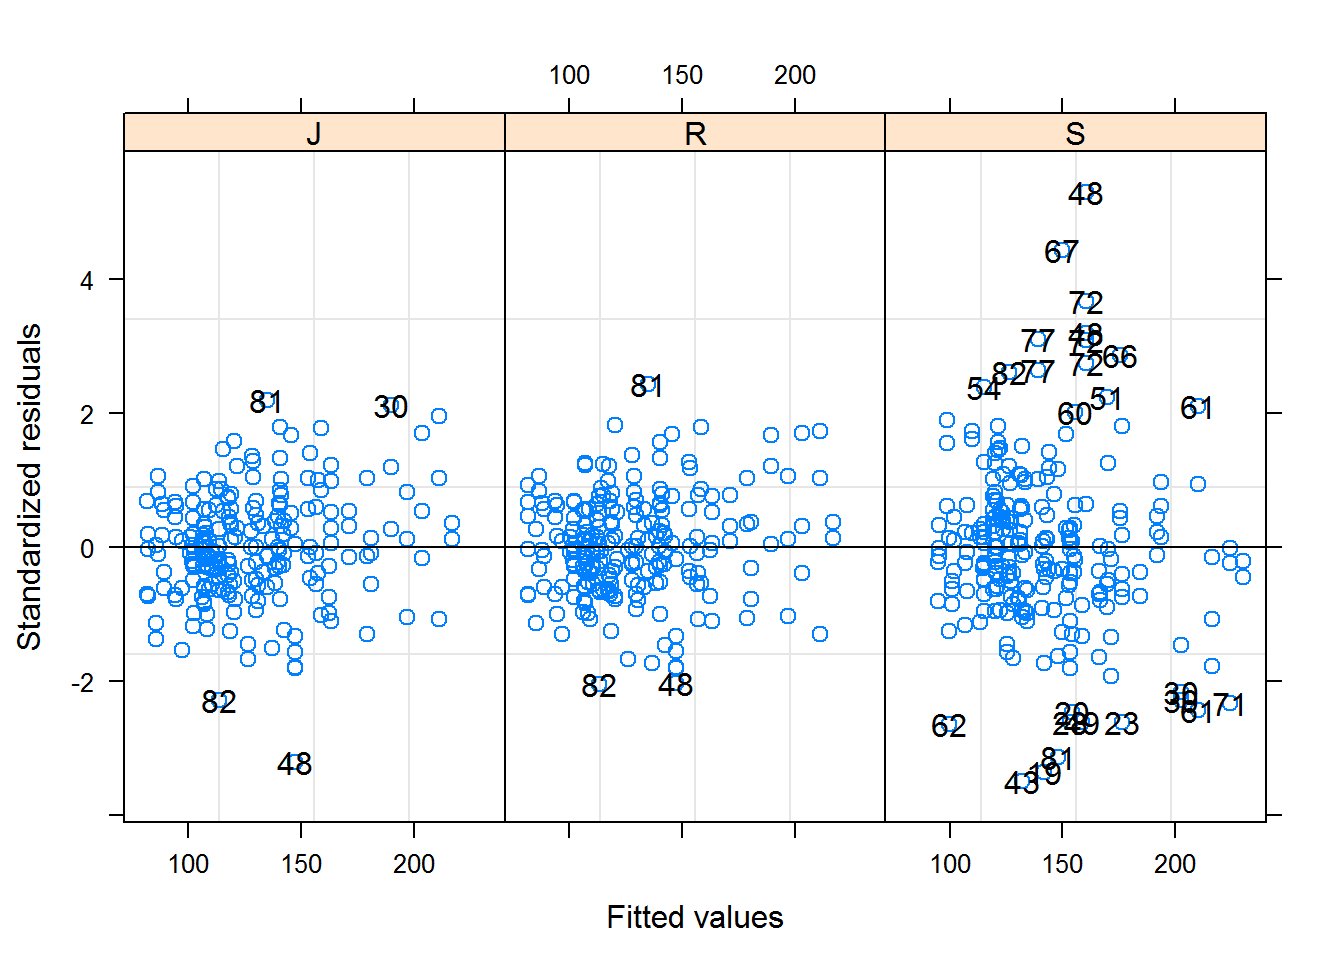
\includegraphics[width=0.9\linewidth]{images/bloodnlmeResidPlot2}
	%		\caption{}
	%		\label{fig:blood}
	%	\end{figure}
	
	\begin{framed}
		\begin{verbatim}
		library(predictMeans)
		CookD(model, group=method, plot=TRUE, idn=5, newwd=FALSE)
		\end{verbatim}
	\end{framed}

	
	
	\begin{framed}
		\begin{verbatim}
		
		blood.red <- blood[!(blood$subject %in% c(68,78,80)),]
		dim(blood.red)
		# 27 observations should be removed.
		
		blood.NLME.red <-lme(BP ~ method-1 , random=~1|subject,data = blood.red)
		plot(blood.NLME.red, resid(., type = "p") ~ fitted(.) | method, abline = 0, id=.05)
		\end{verbatim}
	\end{framed}

	
	\begin{framed}
		\begin{verbatim}
		> shapiro.test(resid(JS.roy1)[1:255])
		
		Shapiro-Wilk normality test
		
		data:  resid(JS.roy1)[1:255]
		W = 0.9931, p-value = 0.2852
		\end{verbatim}
	\end{framed}
	
	\begin{framed}
		\begin{verbatim}
		> shapiro.test(resid(JS.roy1)[256:510])
		
		Shapiro-Wilk normality test
		
		data:  resid(JS.roy1)[256:510]
		W = 0.9395, p-value = 9.503e-09
		\end{verbatim}
	\end{framed}
	%	\begin{figure}[h!]
	%		\centering
	%		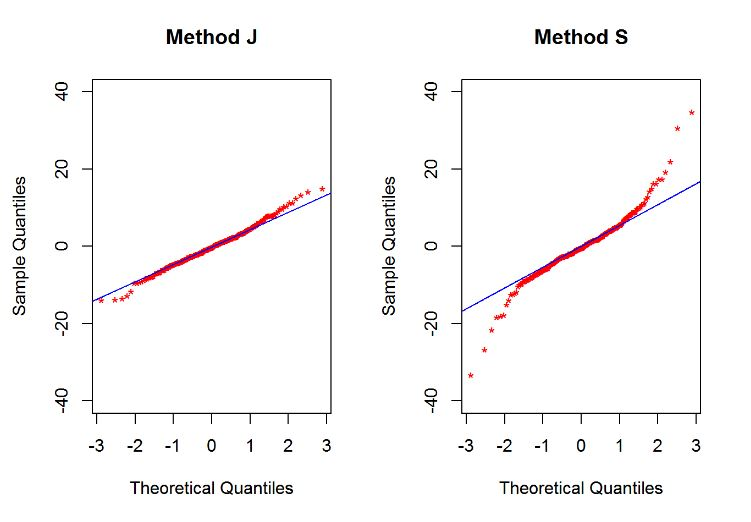
\includegraphics[width=0.9\linewidth]{images/Resid-newplot2}
	%		
	%	\end{figure}
	
	
	
	\begin{framed}
		\begin{verbatim}
		data.frame( response = resid(JS.ARoy20091, type = "response"), 
		pearson  = resid(JS.ARoy20091, type = "pearson"), 
		normalized = resid(JS.ARoy20091, type = "normalized") )
		\end{verbatim}
	\end{framed}
	
	\begin{verbatim}
	response      pearson    normalized
	1    -4.65805902 -0.761587227 -0.7615872269
	2    -0.88701342 -0.145025661  0.0776238081
	3    -5.16580898 -0.844603753 -0.8446037530
	4     2.29041830  0.374480726  0.6450898404
	5     7.87508366  1.287567009  1.2875670086
	6    -6.57048659 -1.074266908 -1.5090772378
	...........................................
	\end{verbatim}
	For the $J$ observations, the variance is 6.116252 whereas for the $S$ observations, the denominator is 9.118144. (with the expected ratio of  1.490806)
	
	
	\begin{framed}
		\begin{verbatim}
		> pearson %>%
		+   as.numeric %>% 
		+   matrix(nrow=85) %>%
		+   round(4) 
		[,1]    [,2]    [,3]    [,4]    [,5]    [,6]
		[1,] -0.7616  0.2194  0.3829 -0.2983  0.3597 -0.0790
		[2,] -0.1450  0.1820 -0.1450 -0.5014  0.1567  0.2663
		[3,] -0.8446  0.4634  0.1364 -0.1630 -0.2727  0.1660
		[4,]  0.3745 -0.2795 -0.2795 -0.2658 -0.2658  0.6115
		[5,]  1.2876 -0.6744 -0.6744  0.8935 -0.0935 -0.8612
		[6,] -1.0743  1.8687 -0.7473 -0.0383  0.2908 -0.3673
		...........................................
		
		\end{verbatim}
	\end{framed}
	
	We can plot the residuals against the fitted values, to assess the assumption of constant variance. 
	\begin{framed}
		\begin{verbatim}
		# standardized residuals versus fitted values 
		plot(JS.ARoy20091, resid(., type = "pearson") ~ fitted(.) , 
		abline = 0, id = 0.05)
		\end{verbatim}
	\end{framed}
	
	
	\begin{framed}
		\begin{verbatim}
		par(mfrow=c(1,2))
		qqnorm((resid(JS.ARoy20091)[1:255]),
		pch="*",col="red",
		ylim=c(-40,40),
		main="Method J")
		qqline(resid(JS.ARoy20091)[1:255],col="blue")
		qqnorm((resid(JS.ARoy20091)[256:510]),
		pch="*",col="red",
		ylim=c(-40,40),
		main="Method S")
		qqline(resid(JS.ARoy20091)[256:510],col="blue")
		par(mfrow=c(1,1))
		\end{verbatim}	
	\end{framed}
	
	\subsubsection{Residuals plots}
	

	
	When the \texttt{plot} function calls the model object, the residual plot is produced.
	
	
	%====================================================================%
	
	
	\begin{framed}
		\begin{verbatim}
		plot(JS.roy1, which=c(1) )
		\end{verbatim}
	\end{framed}
	
	LME models assume that the residuals of the model are normally distributed. A Normal probability plot can be constructed to check this assumption. Commonly used \texttt{R} commands can be used to construct the plot.
	
	
	\begin{framed}
		\begin{verbatim}
		qqnorm(resid(JS.roy1),pch="*",col="red")
		qqline(resid(JS.roy1),col="blue")
		\end{verbatim}
	\end{framed}
	
	\begin{framed}
		\begin{verbatim}
		table(dat$method[1:255])
		## 
		##   J   S 
		## 255   0
		table(dat$method[256:510])
		## 
		##   J   S 
		##   0 255
		\end{verbatim}	
	\end{framed}

	\begin{framed}
		\begin{verbatim}
		plot(roy.NLME, resid(., type = "p") ~ fitted(.) | method, 
		abline = 0, id=.05)
		\end{verbatim}
	\end{framed}
	%	\begin{figure}
	%		\centering
	%		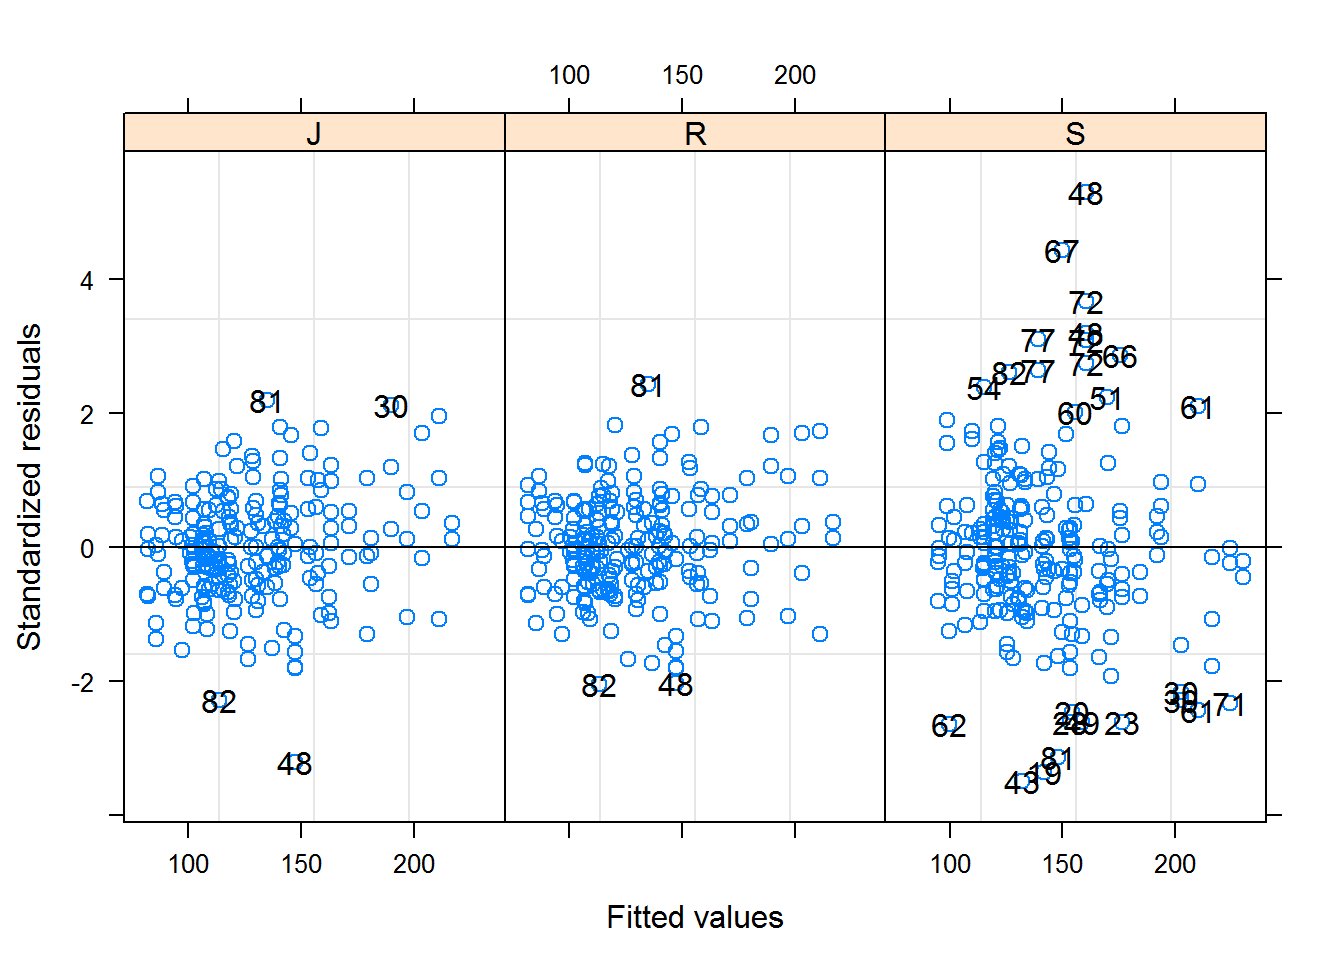
\includegraphics[width=0.9\linewidth]{images/bloodnlmeResidPlot2}
	%		\caption{}
	%		\label{fig:blood}
	%	\end{figure}
	

	
	
	
	\begin{framed}
		\begin{verbatim}
		data.frame( response = resid(JS.ARoy20091, type = "response"), 
		pearson  = resid(JS.ARoy20091, type = "pearson"), 
		normalized = resid(JS.ARoy20091, type = "normalized") )
		\end{verbatim}
	\end{framed}
	
	\begin{verbatim}
	response      pearson    normalized
	1    -4.65805902 -0.761587227 -0.7615872269
	2    -0.88701342 -0.145025661  0.0776238081
	3    -5.16580898 -0.844603753 -0.8446037530
	4     2.29041830  0.374480726  0.6450898404
	5     7.87508366  1.287567009  1.2875670086
	6    -6.57048659 -1.074266908 -1.5090772378
	...........................................
	\end{verbatim}
	For the $J$ observations, the variance is 6.116252 whereas for the $S$ observations, the denominator is 9.118144. (with the expected ratio of  1.490806)
	
	
	\begin{framed}
		\begin{verbatim}
		> pearson %>%
		+   as.numeric %>% 
		+   matrix(nrow=85) %>%
		+   round(4) 
		[,1]    [,2]    [,3]    [,4]    [,5]    [,6]
		[1,] -0.7616  0.2194  0.3829 -0.2983  0.3597 -0.0790
		[2,] -0.1450  0.1820 -0.1450 -0.5014  0.1567  0.2663
		[3,] -0.8446  0.4634  0.1364 -0.1630 -0.2727  0.1660
		[4,]  0.3745 -0.2795 -0.2795 -0.2658 -0.2658  0.6115
		[5,]  1.2876 -0.6744 -0.6744  0.8935 -0.0935 -0.8612
		[6,] -1.0743  1.8687 -0.7473 -0.0383  0.2908 -0.3673
		...........................................
		
		\end{verbatim}
	\end{framed}
	
	We can plot the residuals against the fitted values, to assess the assumption of constant variance. 
	\begin{framed}
		\begin{verbatim}
		# standardized residuals versus fitted values 
		plot(JS.ARoy20091, resid(., type = "pearson") ~ fitted(.) , 
		abline = 0, id = 0.05)
		\end{verbatim}
	\end{framed}
	
	
	\begin{framed}
		\begin{verbatim}
		par(mfrow=c(1,2))
		qqnorm((resid(JS.ARoy20091)[1:255]),
		pch="*",col="red",
		ylim=c(-40,40),
		main="Method J")
		qqline(resid(JS.ARoy20091)[1:255],col="blue")
		qqnorm((resid(JS.ARoy20091)[256:510]),
		pch="*",col="red",
		ylim=c(-40,40),
		main="Method S")
		qqline(resid(JS.ARoy20091)[256:510],col="blue")
		par(mfrow=c(1,1))
		\end{verbatim}	
	\end{framed}
	
	This code will allow you to make QQ plots for each level of the random effects.  LME models assume that not only the within-cluster residuals are normally distributed, but that each level of the random effects are as well. Depending on the model, you can vary the level from 0, 1, 2 and so on
	\begin{framed}
		\begin{verbatim}
		qqnorm(JS.ARoy20091, ~ranef(.))
		
		# 	qqnorm(JS.ARoy20091, ~ranef(.,levels=1)
		\end{verbatim}
	\end{framed}
	\begin{figure}[h!]
		\centering
		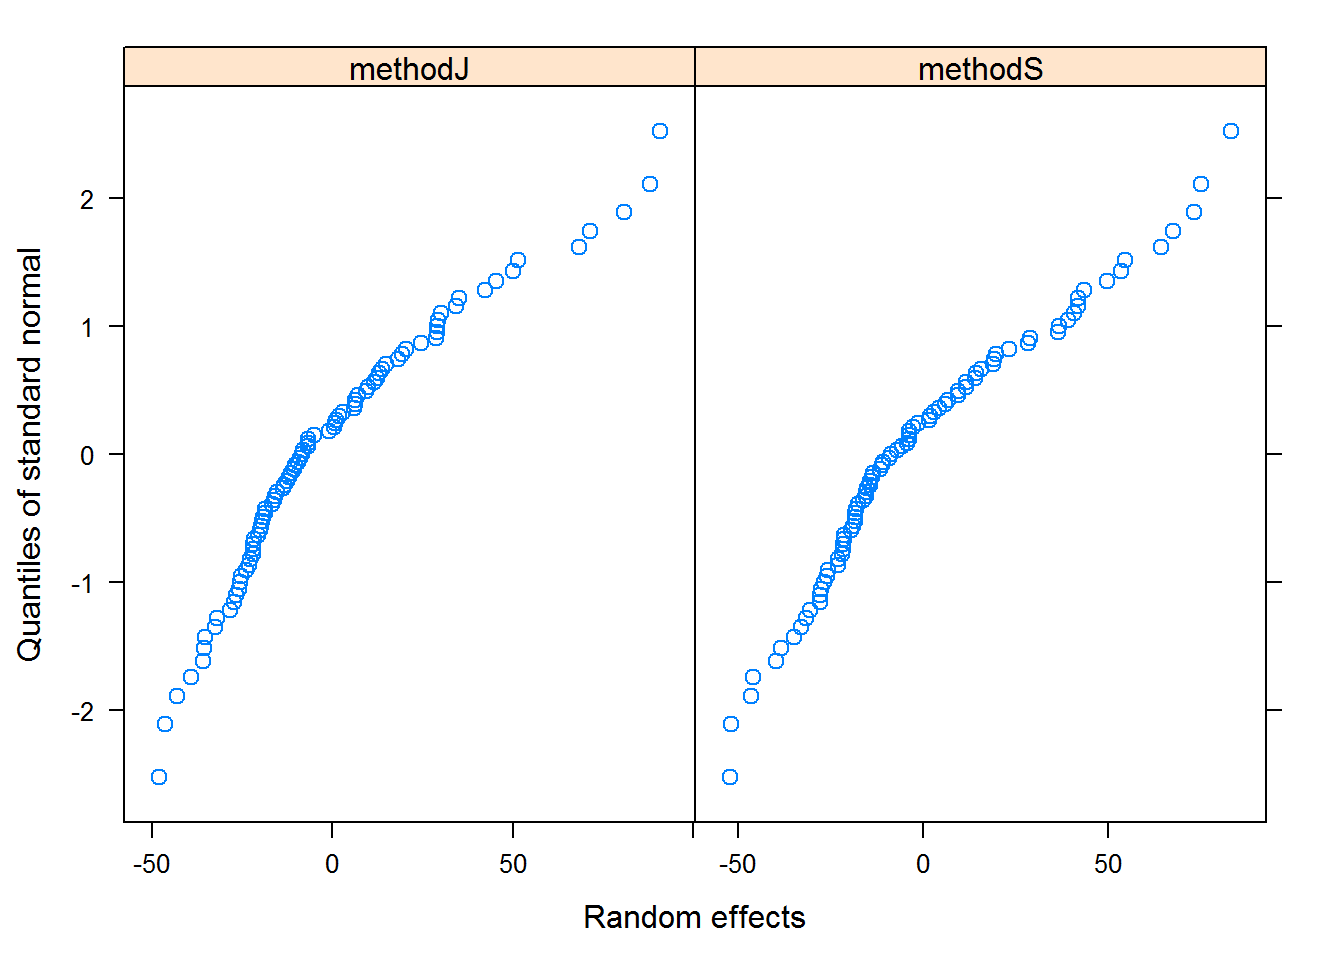
\includegraphics[width=0.9\linewidth]{images/ResidPlot2}
		\caption{}
		\label{fig:ResidPlot2}
	\end{figure}	
	
	
	\begin{framed}
		\begin{verbatim}
		data.frame( response = resid(JS.roy1, type = "response"), 
		pearson  = resid(JS.roy1, type = "pearson"), 
		normalized = resid(JS.roy1, type = "normalized") )
		\end{verbatim}
	\end{framed}
	
	\begin{verbatim}
	response      pearson    normalized
	1    -4.65805902 -0.761587227 -0.7615872269
	2    -0.88701342 -0.145025661  0.0776238081
	3    -5.16580898 -0.844603753 -0.8446037530
	4     2.29041830  0.374480726  0.6450898404
	5     7.87508366  1.287567009  1.2875670086
	6    -6.57048659 -1.074266908 -1.5090772378
	...........................................
	\end{verbatim}
	For the $J$ observations, the variance is 6.116252 whereas for the $S$ observations, the denominator is 9.118144. (with the expected ratio of  1.490806)
	
	
	\begin{framed}
		\begin{verbatim}
		> pearson %>%
		+   as.numeric %>% 
		+   matrix(nrow=85) %>%
		+   round(4) 
		[,1]    [,2]    [,3]    [,4]    [,5]    [,6]
		[1,] -0.7616  0.2194  0.3829 -0.2983  0.3597 -0.0790
		[2,] -0.1450  0.1820 -0.1450 -0.5014  0.1567  0.2663
		[3,] -0.8446  0.4634  0.1364 -0.1630 -0.2727  0.1660
		[4,]  0.3745 -0.2795 -0.2795 -0.2658 -0.2658  0.6115
		[5,]  1.2876 -0.6744 -0.6744  0.8935 -0.0935 -0.8612
		[6,] -1.0743  1.8687 -0.7473 -0.0383  0.2908 -0.3673
		...........................................
		
		\end{verbatim}
	\end{framed}
	
	We can plot the residuals against the fitted values, to assess the assumption of constant variance. 
	\begin{framed}
		\begin{verbatim}
		# standardized residuals versus fitted values 
		plot(JS.roy1, resid(., type = "pearson") ~ fitted(.) , 
		abline = 0, id = 0.05)
		\end{verbatim}
	\end{framed}
	\begin{figure}[h!]
		\centering
		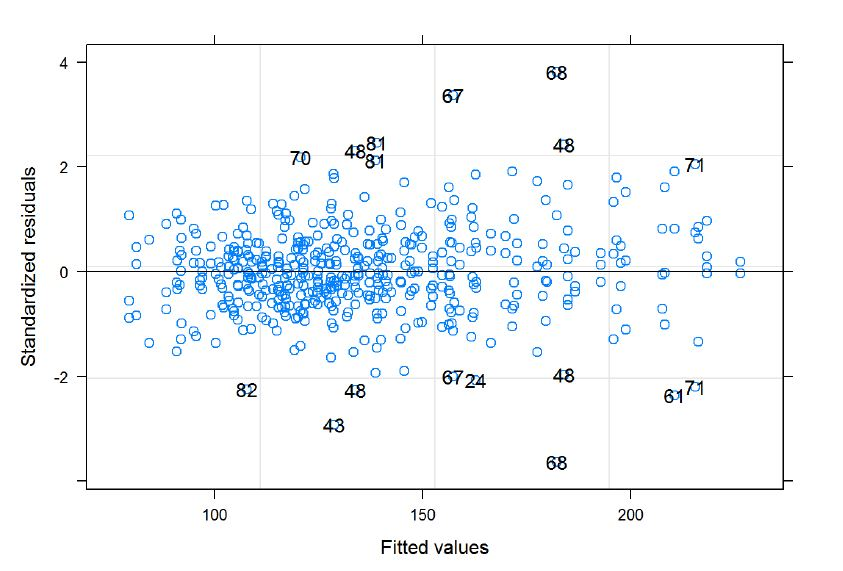
\includegraphics[width=0.9\linewidth]{images/Residuals-JS-Roy}
		\caption{}
		\label{fig:Residuals-JS-Roy}
	\end{figure}
	

\begin{itemize}
	\item
	The \textbf{Scale-Location} plot, also called ‘Spread-Location’ or ‘S-L’ plot, takes the square root of the absolute residuals in order to diminish skewness (sqrt(|E|)) is much less skewed than | E | for Gaussian zero-mean E).
	
	\item
	The \textbf{Residual-Leverage} plot shows contours of equal Cook's distance, for values of cook.levels (by default 0.5 and 1) and omits cases with leverage one with a warning. If the leverages are constant (as is typically the case in a balanced aov situation) the plot uses factor level combinations instead of the leverages for the x-axis. (The factor levels are ordered by mean fitted value.)
\end{itemize}
\begin{framed}
	\begin{verbatim}
	par(mfrow=c(4,1))
	plot(fittedmodel)
	par(opar)
	\end{verbatim}
\end{framed}

%---------------------------------------------------------------------------%
\chapter{Residuals for LME Models}
	%-------------------------------------------------------------- %
	

\section{Diagnostic Tools for the nlme package}


With the nlme package, the generic function \texttt{lme()} fits a linear mixed-effects model in the formulation described in Laird and Ware (1982) but allowing for nested random effects. 

The within-group errors are allowed to be correlated and/or have unequal variances, which is very important in fitting the models for Roy's Tests

The nlme package has a limited set of diagnostic tools that can be used to assess the model fit. A review of the package manual is sufficient to get a sense of the package's capability in that regard.




\section{Computation and Notation } %2.3
with $\boldsymbol{V}$ unknown, a standard practice for estimating $\boldsymbol{X \beta}$ is the estime the variance components $\sigma^2_j$,
compute an estimate for $\boldsymbol{V}$ and then compute the projector matrix $A$, $\boldsymbol{X \hat{\beta}}  = \boldsymbol{AY}$.


%\citet{zewotir} remarks that $\boldsymbol{D}$ is a block diagonal with the $i-$th block being $u \boldsymbol{I}$



%-------------------------------------------------------------------------------------------------Chapter 3------------------------%
%-------------------------------------------------------------------------------------------------------------------------------------%
%-------------------------------------------------------------------------------------------------------------------------------------%


\chapter{Application to Method Comparison Studies} % Chapter 4


%---------------------------------------------------------------------------%
% - 1. Application to MCS
% - 2. Grubbs' Data
% - 3. R implementation
% - 4. Influence measures using R


%\printindex
%\bibliographystyle{chicago}
%\bibliography{DB-txfrbib}
\end{document}